\documentclass[11pt,spanish,a4paper]{article}
% Versión 1.er cuat 2017 Víctor Bettachini < victorb@gmx.net >

\usepackage{babel}
\addto\shorthandsspanish{\spanishdeactivate{~<>}}
\usepackage[utf8]{inputenc}

\usepackage{float}

%% unidades, isótopos, notación física
\usepackage[locale=FR, per-mode=fraction, separate-uncertainty=true]{siunitx}
\sisetup{detect-all}
%\DeclareSIUnit\torr{torr}
%\DeclareSIUnit\atm{atm}
%\usepackage{isotope} % $\isotope[A][Z]{X}\to\isotope[A-4][Z-2]{Y}+\isotope[4][2]{\alpha}$
\usepackage[arrowdel]{physics}

\usepackage{amsmath}
\usepackage{amstext}
\usepackage{amssymb}

\usepackage{booktabs} % table rules

\usepackage{graphicx}
\graphicspath{{./graphs/}}

\usepackage{tikz}
\usetikzlibrary{decorations.pathmorphing}
\usetikzlibrary{patterns}
% \input{DimLinesTikz}

\usepackage[margin=1.3cm,nohead]{geometry}

\usepackage{lastpage}
\usepackage{fancyhdr}
\pagestyle{fancyplain}
\fancyhead{}
% \fancyfoot{{\tiny \textcopyright V. A. Bettachini}}
\fancyfoot{{Víctor A. Bettachini}}
% \fancyfoot{{\tiny \textcopyright Universidad Provincial de Ezeiza}}
\fancyfoot[C]{ Visualización de datos | TP 1 }
\fancyfoot[R]{ \today}
% \fancyfoot[R]{Pág. \thepage/\pageref{LastPage}}
% \fancyfoot[RO, LE]{Pág. \thepage/\pageref{LastPage}}
\renewcommand{\headrulewidth}{0pt}
\renewcommand{\footrulewidth}{0pt}

\usepackage{hyperref}	% enlaces sin borde rojo y en negro
\hypersetup{ 
    colorlinks=true,
    allcolors= black
}


\usepackage{multicol}	% tablas de multiples columnas



\begin{document}
\begin{center}
  \textsc{\large Trabajo final Visualización}\\
	Grupo 2
\end{center}

\section{Reto VAST 2024}
El objetio del reto anual de tecnología y siencia del análisis visual (Visual Analytics Science and Technology ,VAST), del Instituto de ingeniería eléctrica y electrónica (IEEE) es avanza el cambio a través de la competencia 
Es una actividad realizada en conjunto con la conferencia de visualización VIS de la IEEE.

En su página para el reto de este año se da un contexto ficticio para el reto.
 \cite{noauthor_vast_nodate}.
En un espacio geográfico llamado \emph{Oceanus} donde se produce pesca ilegal.
Una organización sin fines de lucro denominada \emph{FishEye} se enfoca en la problemática.
Han generado un grafo a partir de múltiples fuentes de datos estructurados o no.
Se pide desarrollar herramientas de análisis visual aplicado a gráfos de conocimientos para identificar sesgos, ratrear cambios de comportamiento e inferir patrones temporales.
En un parrafo denominado \emph{Visión de conjunto} se menciona que:
\begin{itemize}
	\item Unas pocas compañías transgreden líneas éticas.
	\item \emph{FishEye} condensó datos de distintas fuentes en \emph{CatchNet, el grafo de conocimiento de Oceanus}.
\end{itemize}

A continuación figuran títulos sobre cuatro distintos mini-retos.
El elegido por este grupo es el tercero.

\section{Mini-reto 3 | Análisis temporal}
En la página principal hay un párrafo dedicado a este reto, que se resume en:
\begin{itemize}
	\item Visualizar cambios en relaciones comerciales en la industria pesquera.
	\item Entender cómo reaccionan las empresas al cierre de un competidor que pesca ilegalmente.
	\item Diseñar visualizaciones para mostrar los cambios e identifiquen empresas que se beneficien de la pesca ilegal.
\end{itemize}

Una sub-página dedicada a este mini-reto da mayor detalle sobre el mismo.
Se divide en tres secciones: trasfondo, tareas y preguntas, pedidos de clarificación y un formulario para envío de trabajos y acceder a los datos.

\subsection{Trasfondo}
Se resume en los siguientes puntos:
\begin{itemize}
	\item Analistas de FishEye trabajan con registros de empresas que muestran:
	\begin{itemize}
		\item propietarios (ownership),
		\item accionistas (shareholders),
		\item transacciones,
		\item productos y servicios típicos de cada entidad
	\end{itemize}
	que se vuelcan al grafo de conocimiento \emph{CatchNet}.
	\item En el último año la empresa \emph{SouthSeafood Express Corp} fue descubierta pescando ilegalmente.
	\item FishEye quiere entender patrones temporales e inferir qué puede estar pasando en el mercado pesquero de Oceanus dado el comportamiento ilegal y el consecuente cierre de \emph{SouthSeafood Express Corp}. 
	\item La naturaleza competitiva del mercado pesquero de Oceanus puede llevar a reacciones agresivas para capturar el negocio de \emph{SouthSeafood Express Corp}
	\item Otra reacciones pueden deberse a la toma de conciencia de que la pesca ilegal no pasa desapercibida.
\end{itemize}


\subsection{Tareas y preguntas}
\emph{FishEye} está interesada en identificar personas que tengan influencia en las redes de negocios.

\begin{description}
	\item[Dinámica de estructuras corporativas]
    FishEye analysts want to better visualize changes in corporate structures over time. Create a visual analytics approach that analysts can use to highlight temporal patterns and changes in corporate structures. Examine the most active people and businesses using visual analytics.
	\item[Transacciones típicas y atípicas]
    Using your visualizations, find and display examples of typical and atypical business transactions (e.g., mergers, acquisitions, etc.). Can you infer the motivations behind changes in their activity?
	\item[Pertenencia e influencia sobre compañías]
		Develop a visual approach to examine inferences. Infer how the influence of a company changes through time. Can you infer ownership or influence that a network may have?
	\item[Redes con \emph{SouthSeafood Express Corp}]
    Identify the network associated with SouthSeafood Express Corp and visualize how this network and competing businesses change as a result of their illegal fishing behavior. Which companies benefited from SouthSeafood Express Corp legal troubles? Are there other suspicious transactions that may be related to illegal fishing? Provide visual evidence for your conclusions.
\end{description}


\section{Datos}
Se provee una base de datos no relacional en formato JSON compatible con la biblioteca de análisis de redes NetworkX \cite{noauthor_networkx_nodate}.% junto con un documento que describe su estructura:
%\begin{itemize}
%	\item \emph{Links} (vértices) 
%\end{itemize}
Un archivo adjunto \verb'VAST2024 - MC3 Data Description.docx' describe la estructura de los mismos:
\begin{verbatim}
VAST 2024 MC3 Data Description
Data dictionary and nodes for MC3:
Graph Description:
    - Directed multi-graph, allowing multiple edges between nodes
    - 60520 nodes
    - 75817 edges
    - 4782 connected components
    - Possible node types are: Person, CEO, Organization, Company, FishingCompany, LogisticsCompany, NewsCompany, FinancialCompany, NGO
    - Possible edge types are: Shareholdership, BeneficialOwnership, WorksFor, FamilyRelationship
    - The graph format is a JSON format generated by Python's network_node_link_data() function. It can likewise be loaded to a networkx object using the corresponding node_link_graph() function. The root-level JSON object consists of graph-level properties specifying that it is directed and a multigraph, a “nodes” key which holds the list of nodes, and a “links” key which holds the list of edges.
Node attributes:
Person nodes (Entity.Person or Entity.Person.CEO)
    - type: The type of node.
    - id: The unique identifier of the node and the name of the person
    - dob: The person's date of birth
    - country: The country associated with the entity. 
Organization nodes (Entity.Organization, Entity.Organization.Company, Entity.Organization.FishingCompany, Entity.Organization.LogisticsCompany, Entity.Organization.NewsCompany, Entity.Organization.FinancialCompany, Entity.Organization.NGO)
    - type: The type of node.
    - id: The unique identifier of the node and the name of the organization
    - country: The country associated with the entity.
    - HeadOfOrg: The head of the organization. Optional.
    - ProductServices: A list of products and services that the organization provides. Optional.
    - TradeDescription: A short description of what the organization does. Optional.
    - PointOfContact: The person the company has listed to contact for questions. Optional.
    - revenue: The last reported annual revenue for the company in local currency; all empty values have been set to 0. Optional.
Edge attributes:
Event.Owns.BeneficialOwnership, Event.Owns.Shareholdership edges, Event.WorksFor edges:
    - type: The type of edge.
    - start_date: The date at which the event began.
    - end_date: The date at which the event ended. This attribute is optional.
FamilyRelationship edges only have type attributes.
Metadata attributes:
Every single node and edge should have each of these fields. 
    - _last_edited_by: The name of the user who last modified this node/edge
    - _last_edited_date: The last time this node/edge was modified
    - _date_added: The day on which this node/edge was first added to the graph
    - _raw_source: The source from which the information was originally obtained
    - _algorithm: The method in which the information was obtained (for this mini-challenge, either automatically imported from pre-existing databases or manually updated by FishEye analysts)
\end{verbatim}


\section{Relaciones de pertenencia en torno a \emph{SouthSeafood Express Corp}}

Una búsqueda manual de menciones de \emph{SouthSeafood Express Corp} en los vértices, nombrados enlaces (links), en la base de datos


En la figura \ref{fig:drawio} 

\begin{figure}[!ht]
	\centering
	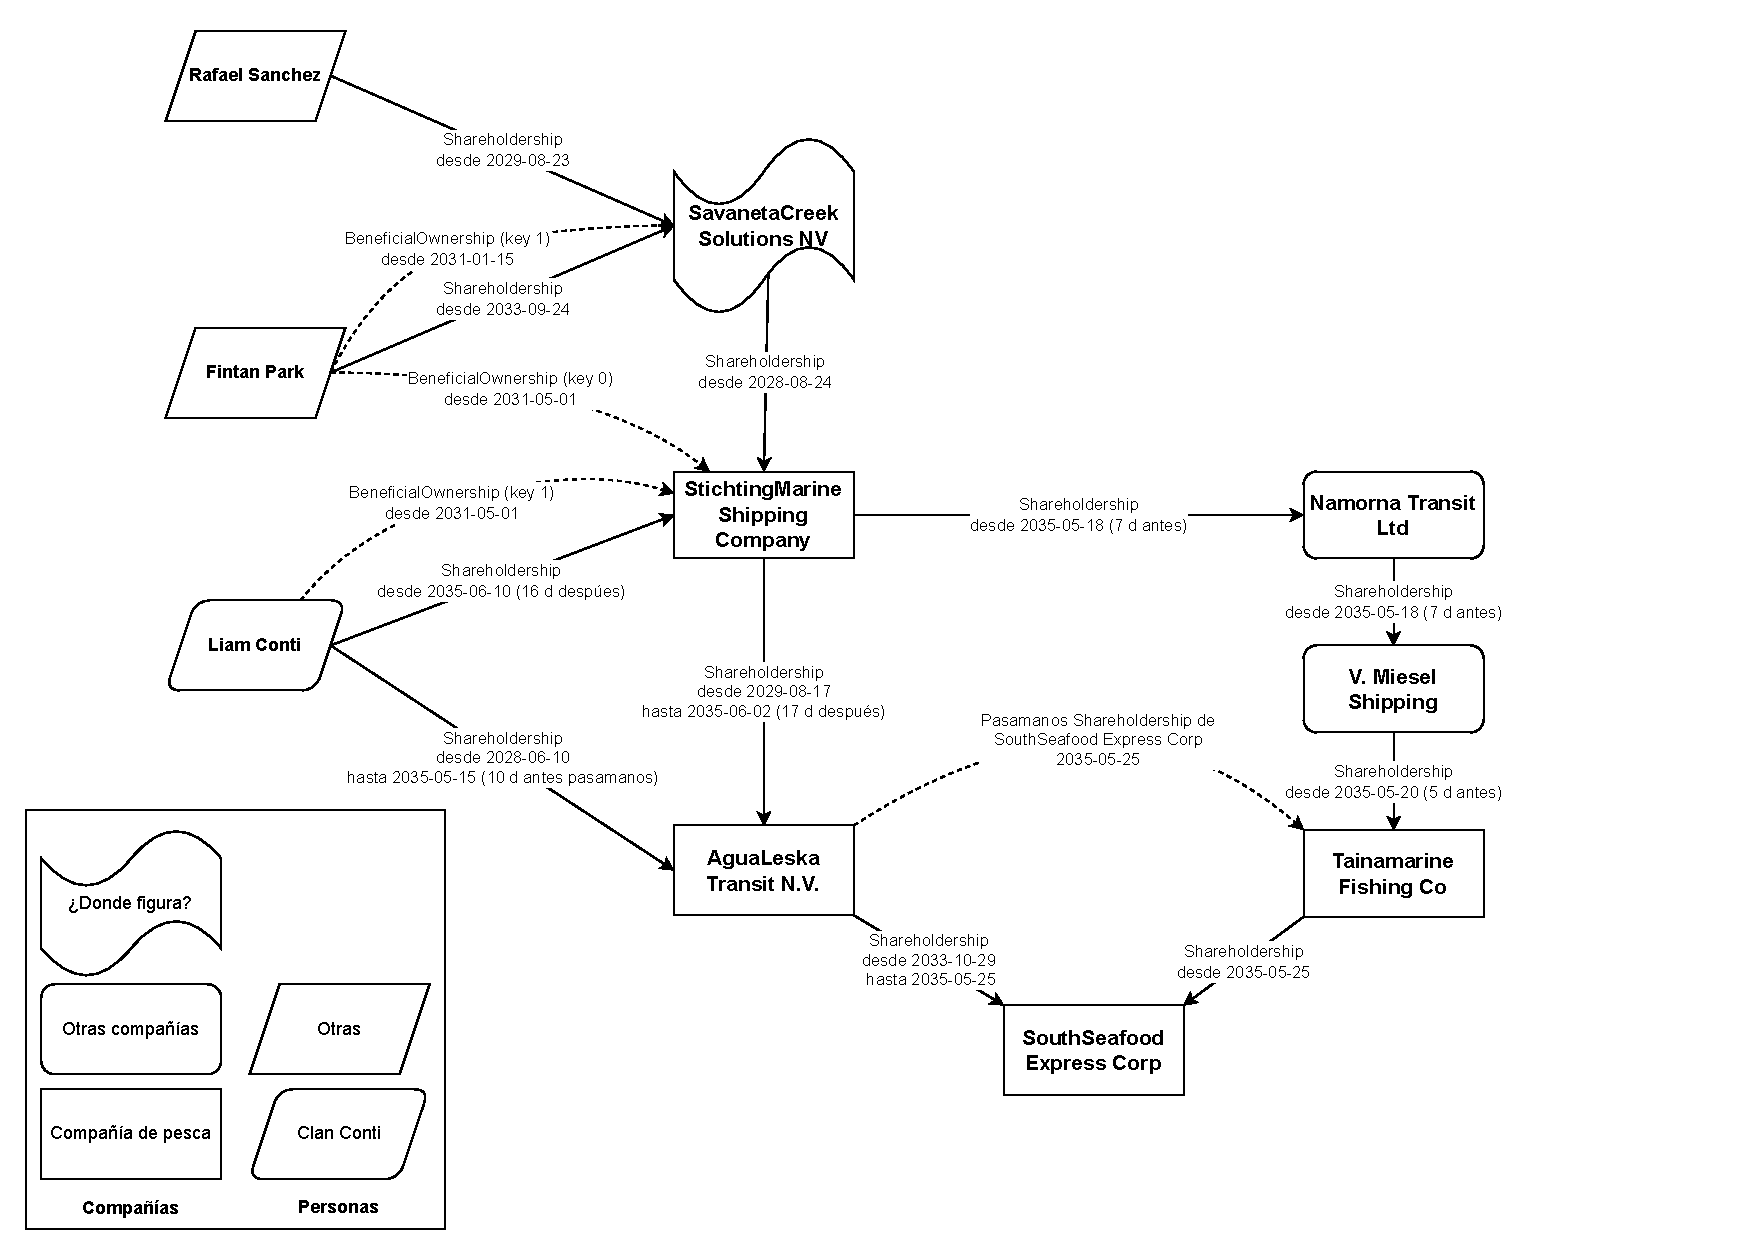
\includegraphics[width=\textwidth]{SouthSeafood.drawio.pdf}
	\caption{Red relaciones en torno a \emph{SouthSeafood Express Corp} generada manualmente siguiendo las relaciones fuente-objetivo en las tablas sobre dueño últiom (\emph{beneficial ownership}) y tenencia de acciones (\emph{share holdership}) de la base de datos.}
	\label{fig:drawio}
\end{figure}



\subsection{Venta de acciones de \emph{SouthSeafood Express Corp}}

Es claro como 

\begin{figure}[!ht]
	\centering
	\begin{subfigure}[b]{\textwidth}
		\centering
		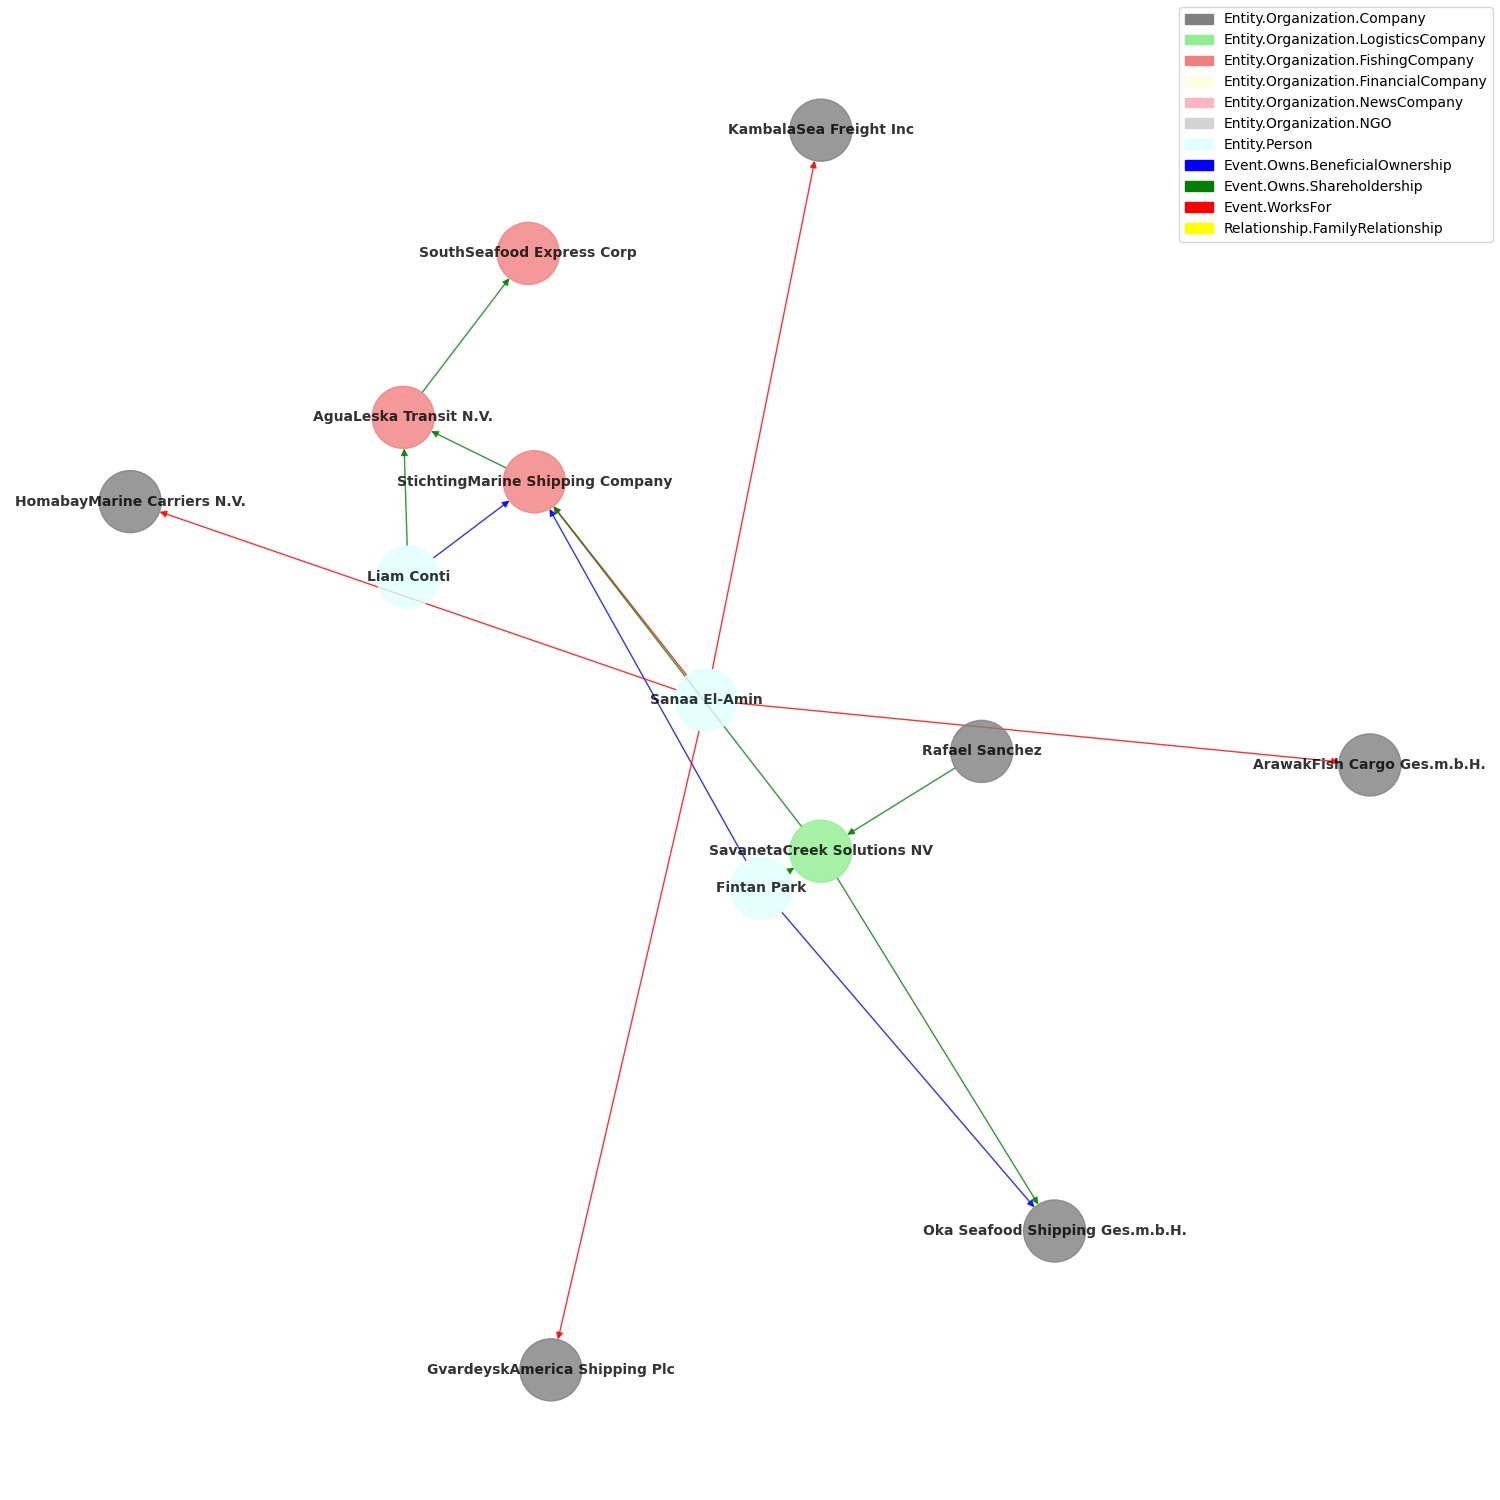
\includegraphics[width=0.6\textwidth]{eins}
		\caption{Al 2025-01-01}
		\label{fig:antes}
	\end{subfigure}
	\begin{subfigure}[b]{\textwidth}
		\centering
		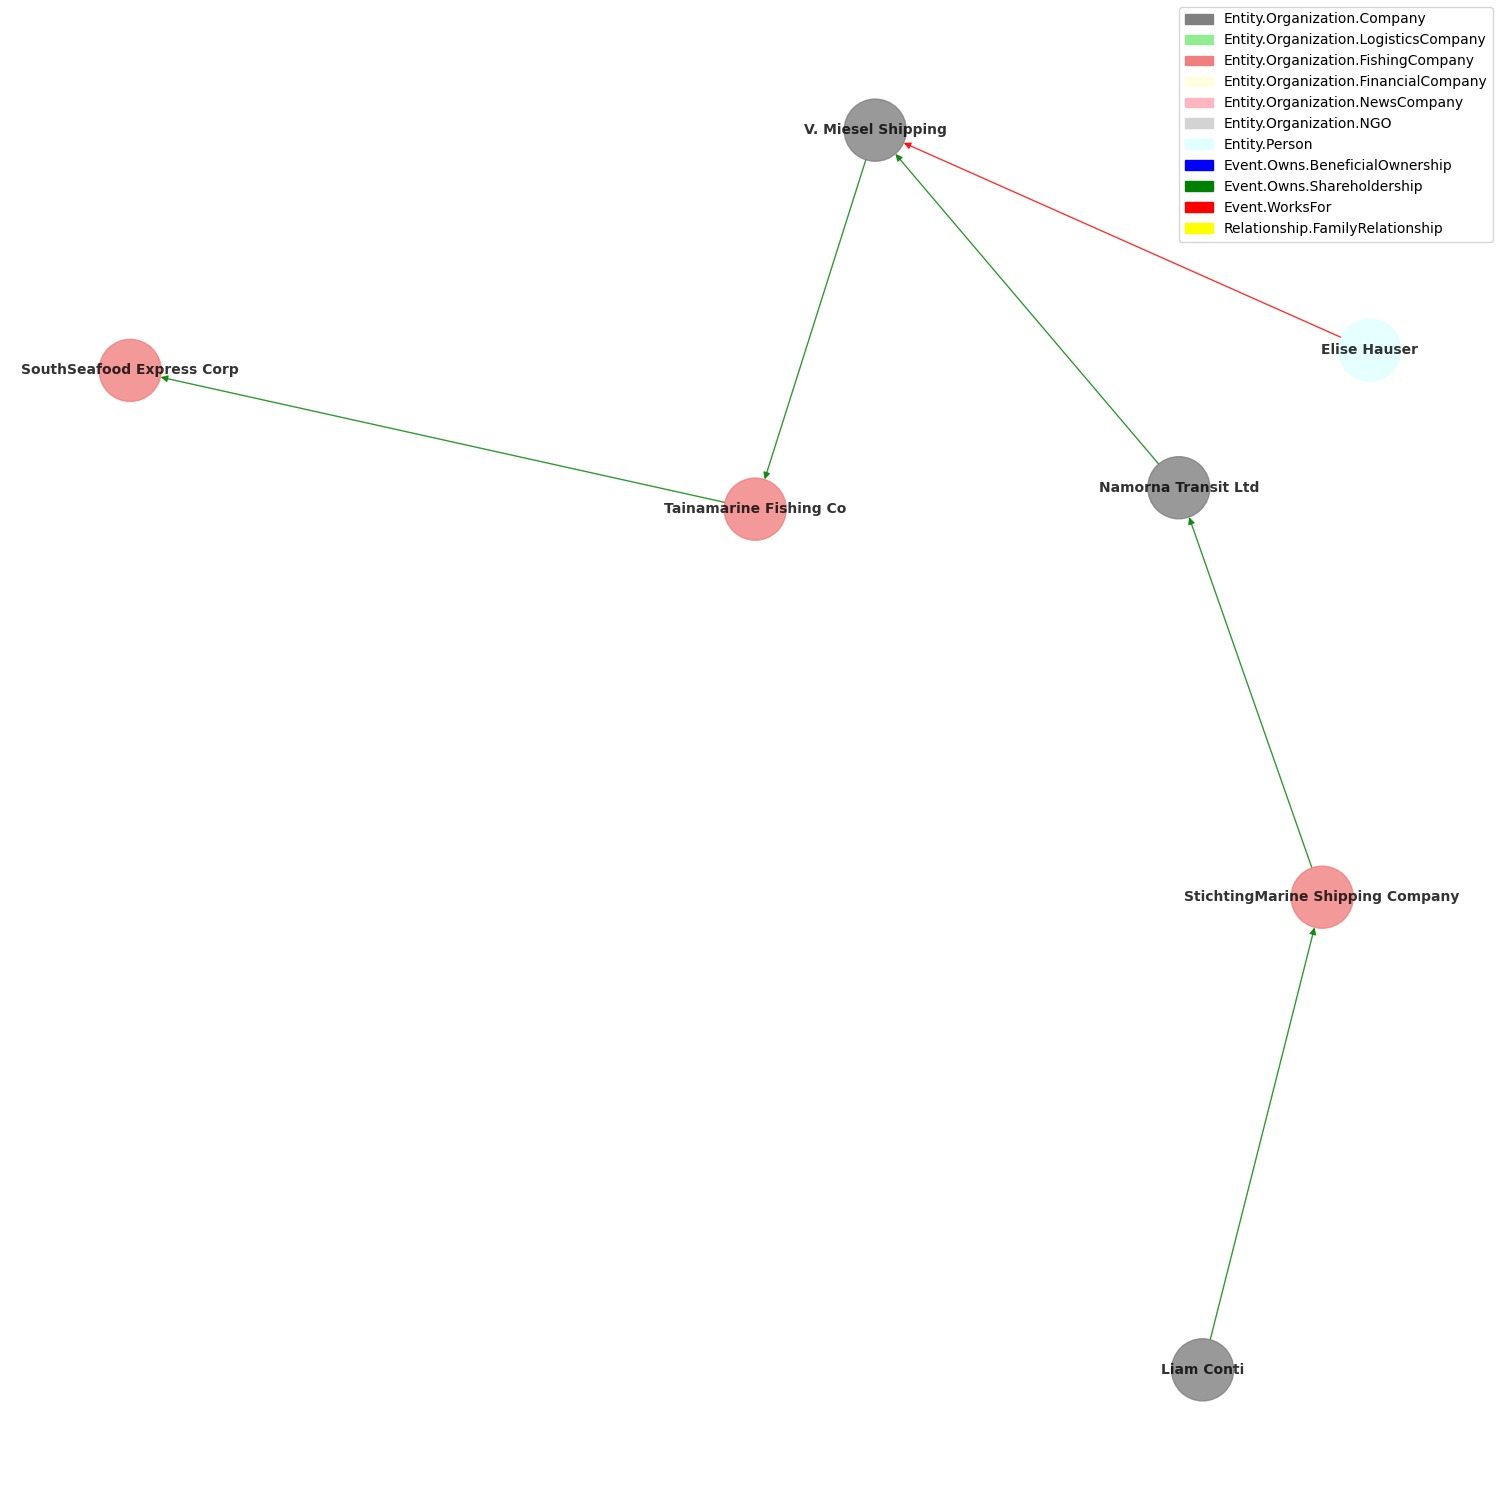
\includegraphics[width=0.6\textwidth]{zwei}
		\caption{Hacía fines de 2025}
		\label{fig:después}
	\end{subfigure}
	\caption{
		Red de relaciónes en toro a \emph{SouthSeafood Express Corp} en 2025-01-01 y hacía fin de ese año.
		La red es orientada por lo que las puntas de las flechas indican el vértice objetivo de cada arista cuyo color indica en apartado de la base de datos figura.
		}
	% \caption{Ahi van dos graficos generados, no fue tan facil como imagine, al final tuve que filtrar por el start_date, pero si tomaba la fecha 25/5 no quedaba grafo para despues asi que puse el 1/1, los anteriores a esa fecha, como era la red de SouthSea antes y los cambios durante el año, incluido varios registros sin start\_date}
	\label{fig:Networkx}
\end{figure}


% \section{Bibliografía}
\printbibliography[heading=bibintoc] % not numbered


\end{document}
